\newpage
\section{Marco teórico}
\subsection{Ferromagnetismo}

El ferromagnetismo es un fenómeno físico (de tipo magnético) que se caractiriza por preservar en el tiempo un comportamiento ordenado de los momentos magnéticos (estado remanente) después de ser aplicado en un campo magnético externo, durante un tiempo suficientemente largo. En dichos materiales, en general, existen regiones, repartidas de forma heterogenea e irregular, donde los espines están orientados en una única dirección (Figura \ref{fig:MagneticDomain}). Este comportamiento se puede describir por la magnetización espontánea, $\mathbf{M}$ \cite{coey_2010}. En el micromagnetismo clásico, la magnitud de la magnetización, para una temperatura fija $T$, es constante \cite{Exl2020} \[ \mathbf{M} (\mathbf{r},T) = |\mathbf{M} (T)| (\gamma_1 (\mathbf{r}) \hat{e}_1 + \gamma_2 (\mathbf{r}) \hat{e}_2 + \gamma_3 (\mathbf{r}) \hat{e}_3 ), \]  es decir, queda totalmente caracterizada por sus cosenos directores $\gamma_i$ referidos a algún sistema ortogonal de coordenadas con vectores unitarios $\hat{e}_k$. 
\begin{figure}[!htp]
    \centering
    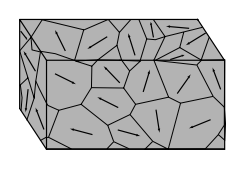
\includegraphics[scale=0.8]{Figuras/MagneticDomain.png}
    \renewcommand{\figurename}{\textbf{Figura}}
    \renewcommand\thefigure{\textbf{\arabic{figure}}}
    \caption{Dominios magnéticos en un sólido ferromagnético \cite{coey_2010}.}
    \label{fig:MagneticDomain}
\end{figure}
\subsection{Términos de energía magnéticos}
En micromagnetismo, la relación básica para el estudio del fenómeno magnético es la densidad de energía libre de Gibbs, $\phi'_l$, la cual se puede escribir como \[ \phi'_l = U - T S - \sigma \cdot \epsilon - \mathbf{J}_s \cdot \mathbf{H}_{ext},\] donde $S$ es la densidad de entropía, $U$ la densidad de energía interna, $\epsilon$ el tensor de estrés y $\mathbf{J}_s$ la polarización espontánea. Además, $U$ contiene los términos de densidad de energía de intercambio, anisotropía magnetocristalina y magnetostática, entre otros. Las variables libres son la temperatura $T$, el tensor elástico $\sigma$ y el campo magnético externo $\mathbf{H}_{ext}$ \cite{KronmüllerMicromagnetism,Exl2020}. La energía libre de Gibbs total en equilibrio térmico está dada por \[ \phi_l = \int \phi'_l ~ dV .\]
\subsubsection{Energía de intercambio}
El Hamiltoniano de intercambio de Heisenberg modela las interacciones de intercambio de los electrones desapareados, usualmente de los átomos vecinos más próximos \cite{coey_2010}, el cual podemos escribir de forma general como \[ \hat{\mathcal{H}}_{ex} = - 2 \sum_{i \neq j} J_{ij} \hat{\mathbf{S}}_i \cdot \hat{\mathbf{S}}_j ,\] donde $J_{ij}$ es la integral de intercambio y $\hat{\mathbf{S}}_k$ son los operadores de espín.

\vspace{10pt}

En el micromagnetismo, la derivación de una expresión continua para las interacciones de intercambio, entre los vecinos más próximos, parte del modelo de Heisenberg. En esta aproximación, se considera a los operadores de espín $\hat{\mathbf{S}}_k$ como vectores clásicos $\mathbf{S}_k$ y el ángulo entre ellos cambia lentamente y de forma continua \cite{Exl2020}. 

\vspace{10pt}

\textbf{Simetrías cúbicas}\\
Para este tipo de simetrías la densidad de energía de intercambio, $\phi'_{ex}$, se puede escribir como \[ \phi'_{ex} = A \sum_{i=1}^3 (\nabla \gamma_i (\mathbf{r}) )^2 ,\] donde $A$ se le conoce como la constante de rigidez de intercambio y puede ser determinada por medio de la expresión \cite{kittel1949} \[ A = \frac{2nJ_0S^2}{a}, \]donde $n$ es el número de átomos por celda unitaria, $J_0$ es la integral de intercambio entre vecinos más proximos, $a$ es el parametro de red y $S$ es la magnitud del vector de espín.

\vspace{10pt}

\textbf{Simetría hexagonal (HCP)}\\
Por otro lado, para las simetrias hexagonales de empaquetamiento compacto (o por sus siglas en inglés, HCP) la constante de rigidez de intercambio toma distintos valores en su componente a lo largo de el eje $c$ ($A_\perp$) y a lo largo del plano basal ($A_\|$) (Figura \ref{fig:hcp}) \cite{KronmüllerMicromagnetism}. Así pues, \[ \phi'_{ex} = A_\perp \sum_{i=1,2} (\nabla \gamma_i (\mathbf{r}) )^2 + A_\| (\nabla \gamma_3 (\mathbf{r}) )^2.\] donde las constantes $A_\perp$ y $A_\|$ se determinan mediante las relaciones \[ A_\perp = \frac{2 J_\perp S^2}{c} \frac{8 \sqrt{3}}{3} \left( \frac{1}{3} + \frac{c^2}{4a^2}  \right) ~~~~~ \land ~~~~~ A_\| = \frac{2 J_\| S^2}{c} \frac{8 \sqrt{3}}{3}.\] 

\subsubsection{Energías magnetostáticas}
La energía magnetostática consta de dos términos: la energía Zeeman y la energía dipolar.

\vspace{10pt}

\textbf{Energía Zeeman}\\
%Añadir que \mu es la permeabilidad magnética del vacio.
La energía Zeeman, o también llamada energía magnetostática del campo externo, surge entre la interacción de los momentos magnéticos electrónicos con un campo externo aplicado \cite{Exl2020}. Se puede expresar la densidad de energía Zeeman como \[ \phi'_H = - \mu_0 \mathbf{H}_{ext} \cdot \mathbf{M},\] donde $\mu_0$ es la permeabilidad magnética del vacio.

\vspace{10pt}

\textbf{Energía Dipolar}\\
En los sólidos cristalinos, cada momento dipolar produce un campo dipolar y cada uno de estos interactúan con el campo producido por los demás dipolos magnéticos, $\mathbf{H}_s$. Como el campo magnético es generado sólo por los momentos dipolares se tiene $\nabla \times \mathbf{H}_s = 0$ y, por tanto, se le puede asociar un potencial escalar, $\mathbf{H}_s = - \nabla U$ \cite{KronmüllerMicromagnetism}. Así pues, la energía dipolar toma la forma \[ \phi_s = \frac{1}{2} \mu_0 \oint_{S_0} \sigma(\mathbf{r}) U(\mathbf{r}) d \mathbf{S} + \frac{1}{2} \mu_0 \int_{V_0} \rho (\mathbf{r}) U(\mathbf{r}) dV ,\] donde $\sigma(\mathbf{r}) = \mathbf{M} (\mathbf{r}) \cdot \hat{\mathbf{n}}$ es la densidad superficial de carga magnética, $\rho(\mathbf{r}) = - \nabla \cdot \mathbf{M} (\mathbf{r})$ la densidad volumétrica de carga magnética y $S_0$ la superficie que contiene al volumen $V_0$ del sistema. Equivalentemente, se puede expresar la densidad de energía dipolar como \[ \phi'_s = \frac{\mu_0}{2} \mathbf{H}_s^2 .\]

\subsubsection{Energía de anisotropía magnetocristalina}
Cuando una o varias propiedades de un material varian con la dirección se dice que dichas propiedades exhiben anisotropía. La anisotropía magnetocristalina es un caso particular de anisotropia magnética, dicho término de energía presenta la misma simetría que la estructura cristalina del material en cuestion \cite{KronmüllerMicromagnetism}. Esta energía está asociada con el hecho de que en los materiales magnéticos existen direcciones para las cuales son fácilmente magnetizables que en otras, esto es, que el campo magnético necesario para magnetizar el material hasta la saturación es menor en unas direcciones que en otras. En la dirección en donde esto sucede decimos que es un ``eje fácil'' y en la dirección de dificil magnetización decimos que es un ``eje duro'' \cite{OHandley}. Una expresión general para la densidad de energía, $\phi'_K$, puede escribirse como \cite{birss1964symmetry} 
\begin{equation}
    \phi'_K = k_0 (\mathbf{r}) + \sum_{i \neq j} k_{ij} \gamma_i (\mathbf{r}) \gamma_j(\mathbf{r}) + \sum_{ijk} k_{ijk} \gamma_i (\mathbf{r}) \gamma_j (\mathbf{r}) \gamma_k (\mathbf{r}) + \dotsc,    \label{eq:anisotropy}
\end{equation}
donde los $k$ son tensores de propiedades del material.

\vspace{10pt}

\textbf{Simetrías cúbicas}\\
Estas estructuras cristalinas tienden a orientar los momentos magneticos en más de un eje fácil, esto se debe a que dichas configuraciones son sumamente simetricas. Para el $\ce{Ni}$, que tiene estructura cubica centrada en las caras (o por sus siglas en inglés, FCC), esta puede orientarse en cuatro distintas direcciones (Figura \ref{fig:niquel}).
\begin{figure}[!hpt]
    \centering
    \begin{subfigure}[b]{0.45\textwidth}
        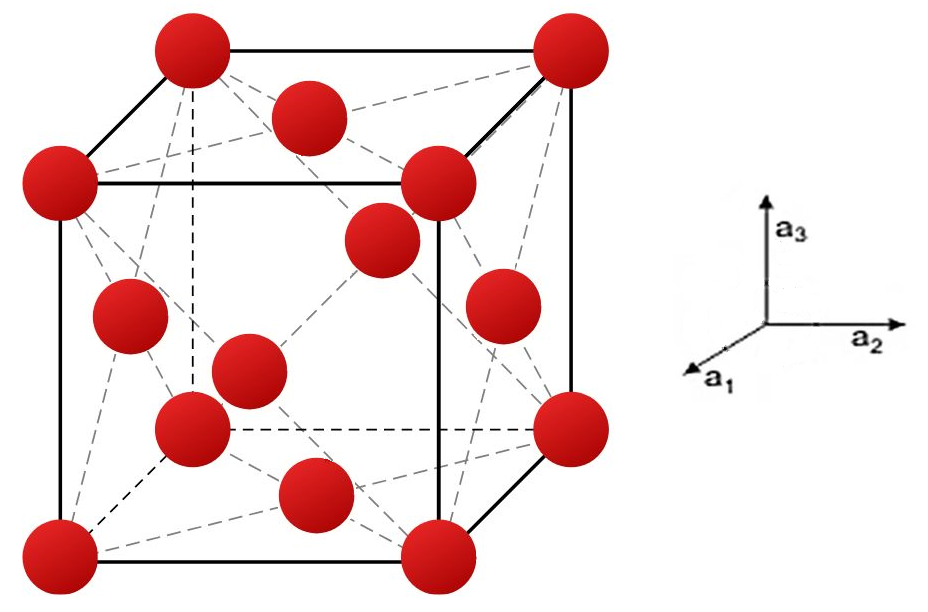
\includegraphics[scale=0.45]{Figuras/Crystal-fcc.png}
        \caption{}
        \label{fig:fcc}
    \end{subfigure}
    \begin{subfigure}[b]{0.4\textwidth}
        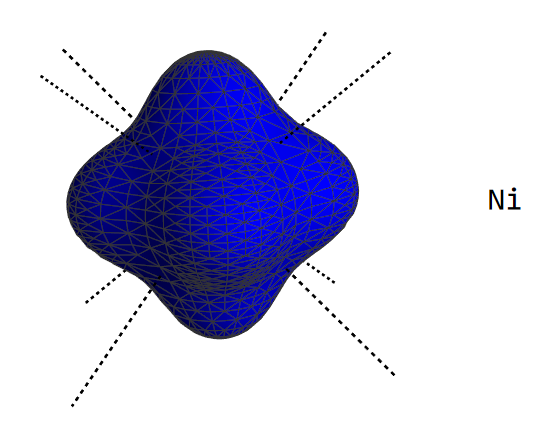
\includegraphics[scale=0.35]{Figuras/MagnetocrystallineNi.png}
        \caption{}
        \label{fig:anisotropyfcc}
    \end{subfigure}
    \renewcommand{\figurename}{\textbf{Figura}}
    \renewcommand\thefigure{\textbf{\arabic{figure}}}
    \caption{a) Estructura cristalina del $\ce{Ni}$. b) Superficie de energía de anisotropía magnetocristalina para el $\ce{Ni}$.}
    \label{fig:niquel}
\end{figure}

Una expresión general para las simetrías cúbicas se deriva a partir de la ecuación \ref{eq:anisotropy}, donde el $\ce{Ni}$ se caractiza por tener una constante $k_2$ negativa. Así pues, \[ \phi'_K = k_0 + k_1 (\gamma_1^2 (\mathbf{r})\gamma_2^2 (\mathbf{r})+\gamma_1^2 (\mathbf{r})\gamma_3^2 (\mathbf{r}) +\gamma_2^2 (\mathbf{r})\gamma_3^2 (\mathbf{r})) + k_2 \gamma_1^2 (\mathbf{r})\gamma_2^2 (\mathbf{r}) \gamma_3^2 (\mathbf{r}) + \dotsc \]

\vspace{10pt}

\textbf{Simetría hexagonal (HCP)}\\
En este tipo de simetrías cristalograficas, presentes en el $\ce{Co}$, la magnetización tiende a alianerse sobre un único eje, esto es, que la magnetización tiende a aliarse sobre la dirección $c$ $([0001])$ en la estructura HCP (Figura \ref{fig:uniaxialhcp}). Cuando la anisotropía magnetocristalina tiene un único eje fácil decimos que presenta anisotropía uniaxial.

\begin{figure}[!hpt]
    \centering
    \begin{subfigure}[b]{0.45\textwidth}
        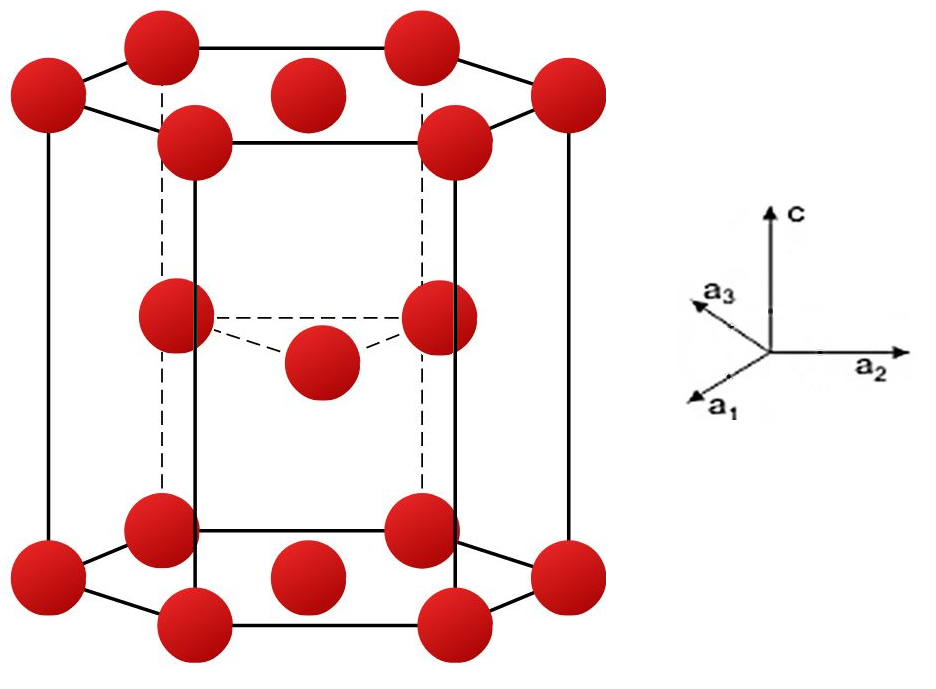
\includegraphics[scale=0.20]{Figuras/Crystal-hcp.png}
        \caption{}
        \label{fig:hcp}
    \end{subfigure}
    \begin{subfigure}[b]{0.35\textwidth}
        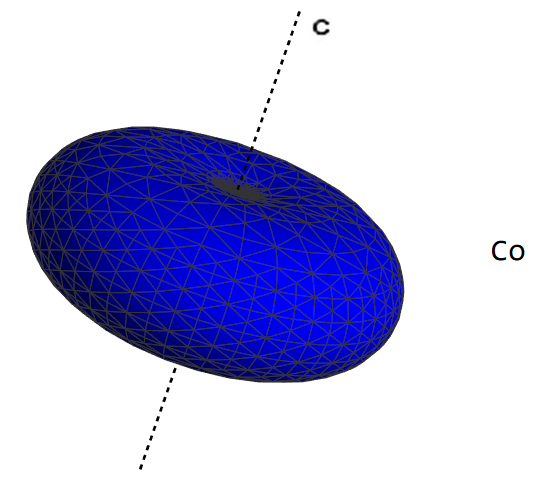
\includegraphics[scale=0.35]{Figuras/MagnetocrystallineCo.png}
        \caption{}
        \label{fig:anisotropyhcp}
    \end{subfigure}
    \renewcommand{\figurename}{\textbf{Figura}}
    \renewcommand\thefigure{\textbf{\arabic{figure}}}
    \caption{a) Estructura cristalina del $\ce{Co}$. b) Superficie de energía de anisotropía magnetocristalina para el $\ce{Co}$.}
    \label{fig:uniaxialhcp}
\end{figure}

Una expresión analitica para la densidad energía de anisotropia se puede derivar a partir de la ecuación \ref{eq:anisotropy} obteniendo así \[ \phi'_K = k_0 + k_1 (\gamma_1^2 (\mathbf{r}) + \gamma_2^2 (\mathbf{r})) + k_2 (\gamma_1^2 (\mathbf{r}) + \gamma_2^2 (\mathbf{r}))^2 + k_3 (\gamma_1^2 (\mathbf{r}) + \gamma_2^2 (\mathbf{r}))^3 + \dotsc \]

\subsection{Ecuaciones de Landau-Lifshitz y Gilbert}
Las ecuaciones LLG describen la evolución en el tiempo de la magnetización espontánea \cite{Exl2020} \[ \frac{d \mathbf{M}}{dt} = \gamma_G (\mathbf{M} \times \mathbf{H}_{eff}) - \frac{\alpha_G}{M}(\mathbf{M} \times \frac{d \mathbf{M}}{dt}),\] donde $\gamma_G$ es la relación giromagnética de los electrones, $\alpha_G$ la constante de amortiguamiento de Gilbert y $\mathbf{H}_{eff} = - (1/J_s) \partial \phi_l / \partial \mathbf{m}$ con $\mathbf{m} = \mathbf{M}/M$ el campo magnético efectivo. 
\subsection{Simulaciones micromagnéticas}
\subsubsection{Métodos numéricos}
Las ecuaciones LLG son un conjunto de ecuaciones no lineales acopladas, por lo que obtener expresiones analíticas puede ser muy laborioso o incluso imposible, así pues, se realizan aproximaciones numéricas para estudiar la dinámica de la magnetización. Los métodos más comunes son el micromagnetismo numérico de diferencias finitas (FE), basado en campo y el basado en energía, y el método de elemento finito (FD). Por un lado, el método FE basado en campo consiste en buscar la solución numérica sobre la base de una evaluación directa de las componentes del campo efectivo $\mathbf{H}_{eff}$ bajo la restricción de las condiciones de frontera. Por otro lado, el método FE basado en energía da prioridad a la energía magnética y se calcula directamente de la magnetización discretizada, mientras que el campo efectivo se deriva de la energía resultante \cite{miltat2007numerical}. Finalmente, el método FD consiste en que el dominio se subdivide en elementos y se aproximan las cantidades de campo usando funciones nodales \cite{FiniteElement}.

\subsubsection{Paquetes principales}
Existen una gran cantidad de paquetes de software de propósito general diseñados para resolver las ecuaciones LLG (Tabla \ref{tab:SoftwarePackage}). A grandes rasgos, las diferencias más importantes de estos paquetes son el método que usan para resolver dichas ecuaciones, el hardware en el que corren (CPU o GPU) y si son de acceso gratuito o comercial \cite{Tomorrow}. Este trabajo de investigación se centra en los dos paquetes de libre acceso más empleados: OOMMF y mumax$^3$.
\begin{table}[htp!]
    \centering
    \resizebox{8cm}{!}{
    \begin{tabular}{|l|c|c|c|}
        \hline
        \textbf{Nombre} & \textbf{FE/FD} & \textbf{CPU/GPU} & \textbf{Gratis} \\ \hline
        LLG & FD & CPU & No \\ \hline
        OOMF & FD & CPU & Si \\ \hline
        micromagus & FD & CPU & No \\ \hline
        magpar & FE & CPU & Si \\ \hline
        Nmag & FE & CPU & Si \\ \hline
        GPMagnet & FD & GPU & No \\ \hline
        FEMME & FE & CPU & No \\ \hline
        tetramaf$^b$ & FE & GPU & No \\ \hline 
        finmag$^c$ & FE & CPU & Si \\ \hline
        Fastmag & FE & GPU & No \\ \hline
        mumax & FD & GPU & Si \\ \hline
        micromagnum & FD & GPU & Si \\ \hline
        magnum.fd$^d$ & FD & GPU & Si \\ \hline
        magnum.fe & FE & CPU & No \\ \hline
        mumax$^3$ & FD & GPU & Si \\ \hline
    \end{tabular}}
    \renewcommand{\tablename}{\textbf{Tabla}}
    \renewcommand\thetable{\textbf{\arabic{table}}}
    \caption{Lista de paquetes de software de propósito general \cite{Tomorrow}.}
    \label{tab:SoftwarePackage}
\end{table}

\subsection{Ciclos de histéresis}
El fenómeno de histéresis consiste en la respuesta no lineal e irreversible de la magnetización con el campo magnético, es decir, la magnetización no sigue una relación unívoca con el campo y depende, en gran medida, de las características intrínsecas, extrinsecas e historia de preparación del material (Figura \ref{fig:hysteresis}) \cite{coey_2010,jackson2012classical}. Además, en nanohilos cilíndricos, este ciclo de histéresis también está influenciado por la orientación del campo magnético aplicado al mismo \cite{CylindricalMagneticNonowires}.

\begin{figure}[!htp]
    \centering
    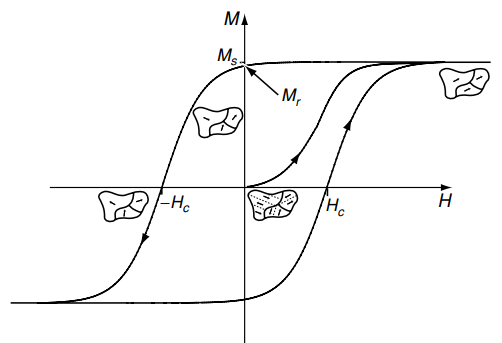
\includegraphics[scale=0.5]{Figuras/Hysteresis.png}
    \renewcommand{\figurename}{\textbf{Figura}}
    \renewcommand\thefigure{\textbf{\arabic{figure}}}
    \caption{Ciclo de histéresis de un ferromagneto. Se observa el comportamiento de los dominios magnéticos cuando es magnetizado hasta la saturación $M_s$, en el estado de magnetización remanente $M_r$ y cuando es aplicado un campo $H_c$ (campo coersitivo) para la anulación de la magnetización \cite{coey_2010}.}
    \label{fig:hysteresis}
\end{figure}

\subsection{Nanohilos ferromagnéticos de Co-Ni con anisotropía transversal}
Este sistema de nanohilos individuales se caracteriza por la aparición de una cadena de vórtices repartidos longitudinalmente en la región $C2$ (Figura \ref{fig:ExoticVortexNW}). En dicha región, el flujo magnético rota alrededor de ejes fijos equidistantes, además, la dirección de giro (horaria o antihoraria) del flujo magnético cambia de forma alternada. En este sistema, conviven dos fases cristalográficas: HCP y FCC, donde se emplea una aleación de $\ce{Co}$-$\ce{Ni}$ con poca concentración de $\ce{Ni}$ para orientar el eje fácil uniaxial, propio de la estructura HCP, perpendicular al eje del nanohilo; de esta manera, se vence la anisotropía de forma que tiende a orientar la magnetización a lo largo del eje del nanohilo \cite{ExoticMagneticConfiguration}. Por otro lado, este tipo de sistemas magnéticos pueden tener aplicaciones tecnologías interasantes como: memorias magnéticas, debido a que se puede llegar a manipular deliberadamente la polaridad del arreglo de vórtices lo que puede ser usado para el desarrollo de dispositivos de almacenamiento extremadamente compactos; o circutos lógicos, ya que esta cadena puede ser controlada mediante corrientes o campos externos \cite{FieldTuneble}.
\begin{figure}[!hpt]
    \centering
    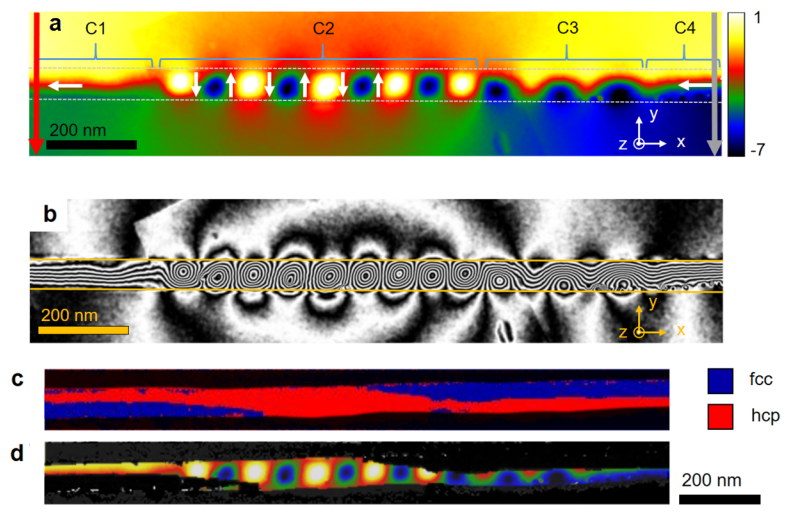
\includegraphics[scale=0.7]{Figuras/ExoticVortexNW.png}
    \renewcommand{\figurename}{\textbf{Figura}}
    \renewcommand\thefigure{\textbf{\arabic{figure}}}
    \caption{La figura a) muestra el cambio de fase magnética y b) muestra las lineas de flujo magnetico. Las gráficas c) y d) corresponden a resultados experimentales del analisis estructural del nanohilo. La Figura c) muestra las fases cristalográficas FCC y HCP en la dirección $z$ al eje del nanohilo. La figura d) muestra la superposición de las figuras a) y c) en donde solo la fase HCP es visible \cite{ExoticMagneticConfiguration}.}
    \label{fig:ExoticVortexNW}
\end{figure}